% Trying to break the document up a bit.  This command simply inserts the contents of the file at this point.  It contains the document license, preamble, and title page: things that aren't likely to change more than once.  This can be used to separate discrete parts of a document into files that are easier to edit at one time.
%%%%%%%%%%%%%%%%%%%%%%%%%%%%%%%%%%%%%%%%%%%%%%%%%%%%%%%%%%%%%%%%%%%%%%
% This layout was adapted from one found at latextemplates.com which
% was adapted from another.
%
% License: CC BY-NC-SA 3.0
% (http://creativecommons.org/licenses/by-nc-sa/3.0/)
%
% Original header:
%
% This is a LaTeX version of the sample laboratory report from
% Virginia Tech's copyrighted 08-09 CHEM 1045/1046 lab manual.
% Reproduction of this one appendix section for academic purposes
% should fall under fair use.
%
%%%%%%%%%%%%%%%%%%%%%%%%%%%%%%%%%%%%%%%%%%%%%%%%%%%%%%%%%%%%%%%%%%%%%%

\documentclass{article}

\usepackage{graphicx}
% \usepackage[acronym]{glossaries} % Lets us use acronyms
\usepackage{multicol}
\usepackage{amsmath}
\usepackage{siunitx} % SI units in math mode
%\usepackage[usenames]{color}
\usepackage{subcaption}

\author{}
\title{ELEC-313 \\ Lab 9: Common-Emitter Transistor Amplifier\\ }
\date{\today}

% \loadglsentries{acronyms} % Actually loads 'acronyms.tex'
% \makeglossaries

\begin{document}

\maketitle

\begin{center}
  \begin{tabular}{lr}
    Date Performed: & November 20, 2013 \\
    Partners:       & Charles Pittman    \\
    & Stephen Wilson     \\
  \end{tabular}
\end{center}

\newpage

%\tableofcontents
%\listoffigures
%\listoftables
%\newpage

% Number the enumerate environment (unordered lists) by letter:
% \renewcommand{\labelenumi}{\alph{enumi}.}

\section{Objective}
\label{sec:objective}


\section{Equipment}
\label{sec:equipment}

\begin{tabular}{ll}
  \centering
  Transistor: 2N7000               & Power supply: HP E3631A            \\
  Function generator: HP 33120 & Multimeter: HP 34401A              \\
  Oscilloscope: Agilent 54622D & Capacitors: \SI{0.1}{\micro\farad} \\
  \multicolumn{2}{l}{Resistors: \SI{100}{\ohm}, \SI{300}{\ohm}, \SI{470}{\ohm}, \SI{1}{\kilo\ohm} (x2) \SI{33}{\kilo\ohm}, \SI{100}{\kilo\ohm} (x2)} \\
\end{tabular}

\section{Schematics}
\label{sec:schematics}

% \begin{figure}[hbtp]
%   \centering
%   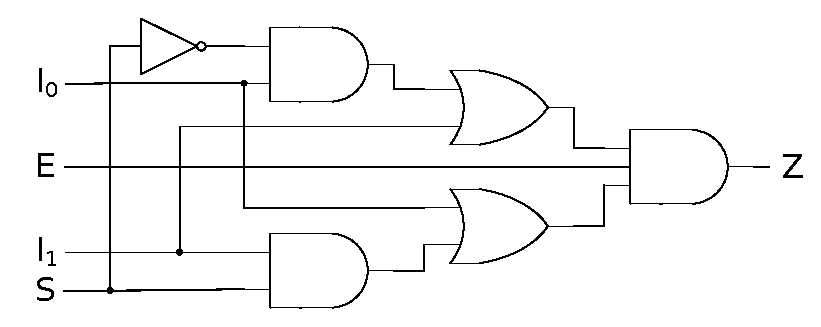
\includegraphics[width=0.6\textwidth]{circuit}
%   \caption{\label{fig:circuit} Circuit used in this lab.}
% \end{figure}

\begin{figure}[hbtp]
  \centering
  \begin{subfigure}[b]{0.4\textwidth}
    \includegraphics[width=\textwidth]{common-source}
    \caption{\label{schem:common-source} Common-source amplifier}
  \end{subfigure}%
  ~
  \begin{subfigure}[b]{0.4\textwidth}
    \includegraphics[width=\textwidth]{source-follower}
    \caption{\label{schem:source-follower} Source-follower amplifier}
  \end{subfigure}
  \caption{\label{fig:schematics} Circuits used in this lab. $R_1=\SI{100}{\kilo\ohm}$,  $R_s=\SI{470}{\ohm}$}
\end{figure}

\section{Procedure}
\label{sec:procedure}

The following procedures were identified to observe the basic operation of MOSFET amplifier circuits.

\subsection{Common-Source Amplifier}

\begin{enumerate}
\item Build the circuit shown in Figure~\ref{schem:common-source}.  Use the closest resistor values available for R1 and Rs.
\item Measure and record the drain current and dc voltages at all terminals of the MOSFET.
\item Set the function generator for a \SI{200}{V_{pp}}, \SI{20}{kHz} sine wave with 0V DC offset.  Connect it to $V_{in}$ .
\item Connect a \SI{100}{\kilo\ohm} load resistor from $V_{out}$ to ground. This will be considered a no-load scenario.
\item Connect channel 1 of the oscilloscope to $V_{in}$ and channel 2 to $V_{out}$ . Set the scope to trigger off of channel 1 . This setting is accessed using the EDGE button on the oscilloscope.
\item Adjust the function generator to an amplitude of \SI{200}{V_{pp}} as measured on channel 1 of the oscilloscope.
\item Measure the peak-to-peak output voltage on channel 2 of the oscilloscope.
\item Repeat step 6 for input voltages (as measured on channel 1 of the oscilloscope) of 300, 400, 500, 600, 700, 800, 900, and \SI{1000}{mV_{pp}} .
\item Replace the \SI{100}{\kilo\ohm} from $V_{out}$ to ground with a \SI{1}{\kilo\ohm} load resistor.
\item Reset the function generator to an amplitude of \SI{200}{V_{pp}} as measured on channel 1 of the oscilloscope.
\item Measure the peak-to-peak output voltage on channel 2 of the oscilloscope.
\end{enumerate}

\subsection{Source-Follower Amplifier}

\begin{enumerate}
\item Construct the circuit shown in Figure~\ref{schem:source-follower} by removing the \SI{1}{\kilo\ohm} drain resistor and moving the output capacitor to the source of the MOSFET.
\item Measure and record the drain current and dc voltages at all terminals of the MOSFET.
\item Connect a \SI{100}{\kilo\ohm} load resistor from $V_{out}$ to ground. This will be considered a no-load scenario.
\item Adjust the function generator to an amplitude of \SI{200}{V_{pp}} as measured on channel 1 of the oscilloscope.
\item Measure the peak-to-peak output voltage on channel 2 of the oscilloscope.
\item Repeat step 4 for input voltages (as measured on channel 1 of the oscilloscope) of 300, 400, 500, 600, 700, 800, 900, and \SI{1000}{mV_{pp}} .
\item Reset the function generator to an amplitude of \SI{200}{V_{pp}} as measured on channel 1 of the oscilloscope.
\item Replace the \SI{100}{\kilo\ohm} resistor from $V_{out}$ to ground with a \SI{1}{\kilo\ohm} resistor and measure the peak-to-peak output voltage on channel 2 of the oscilloscope.
\item Now replace the \SI{1}{\kilo\ohm} load resistor with a 100ohm load resistor and measure the peak-to-peak output voltage on channel 2 of the oscilloscope.
\end{enumerate}

\section{Results}

\subsection{Common-Source Amplifier}

\begin{table}[hbtp]
  \centering
  \begin{tabular}{cccc}
    $V_G$ & $V_D$ & $V_S$ & $I_D$ \\
    \hline
    \SI{4.391}{V} & \SI{13.498}{V} & \SI{2.11}{V} & \SI{4.52}{mA} \\
  \end{tabular}
  \caption{\label{tab:tran_common} Transistor characteristics}
\end{table}

\begin{table}[hbtp]
  \centering
  \begin{tabular}{cc}
    $V_{in}$ (\si{mV}) & $V_{out}$ (\si{V}) \\
    \hline
    200          & 0.382         \\
    300          & 0.566         \\
    400          & 0.760         \\
    500          & 0.939         \\
    600          & 1.140         \\
    700          & 1.340         \\
    800          & 1.530         \\
    900          & 1.721         \\
    1000         & 1.90          \\
  \end{tabular}
  \caption{\label{tab:common-source} Common-source amplifier}
\end{table}

\subsection{Source-Follower Amplifier}

\begin{table}[hbtp]
  \centering
  \begin{tabular}{cccc}
    $V_G$ & $V_D$ & $V_S$ & $I_D$ \\
    \hline
    \SI{4.391}{V} & \SI{18.003}{V} & \SI{2.12}{V} & \SI{4.579}{mA} \\
  \end{tabular}
  \caption{\label{tab:tran_follower} Transistor characteristics}
\end{table}

\begin{table}[hbtp]
  \centering
  \begin{tabular}{cc}
    $V_{in}$ (\si{mV}) & $V_{out}$ (\si{mV}) \\
    \hline
    200                & 182                 \\
    300                & 268                 \\
    400                & 360                 \\
    500                & 451                 \\
    600                & 541                 \\
    700                & 634                 \\
    800                & 725                 \\
    900                & 813                 \\
    1000               & 906                 \\
  \end{tabular}
  \caption{\label{tab:source-follower} Source-follower amplifier}
\end{table}

\begin{table}[hbtp]
  \centering
  \begin{tabular}{ccccc}
    & $V_{G}$ (\si{V}) & $V_{D}$ (\si{V}) & $V_{S}$ (\si{V}) & $I_D$ (\si{mA}) \\
    \hline
    \textbf{Measured} & 4.391 & 13.498 & 2.11 & 4.52 \\
    \textbf{Theoretical} & 4.466 & 14.000 & 2.4214 & 4.00 \\
    \textbf{\% Difference} & 1.712\% & 3.719\% & 14.800\% & 11.500\% \\
  \end{tabular}
  \caption{\label{tab:percent_diff} \% Difference}
\end{table}

\section{Conclusion}
\label{sec:conclusion}


\section{Equations}
\label{sec:equations}

% LaTeX sees blank lines as a start of another paragraph.  To avoid
% unnecessary vertical spaces between equations, and still visually
% separate in source, put a comment between them.
%
\begin{equation}
  \label{eq:amp}
  V_{o,L} = V_{o,NL} \frac{R_L}{R_o + R_L}
\end{equation}
%
\begin{equation}
  \label{eq:V_G}
  V_G = \frac{V_{DD} \cdot \SI{33}{\kilo\ohm}}{\SI{100}{\kilo\ohm} + \SI{33}{\kilo\ohm}}
\end{equation}
%
\begin{equation}
  \label{eq:V_S}
  V_S = V_G \cdot \sqrt{\frac{I_D}{K_N}} - V_{TN}
\end{equation}
%
\begin{equation}
  \label{eq:V_D}
  V_D = V_{DD} - I_D \cdot \SI{1}{\kilo\ohm}
\end{equation}
%
\begin{equation}
  \label{eqn:percent_diff}
  \%_{diff} = \frac{|measured - theoretical|}{theoretical} \times 100\%
\end{equation}

\end{document}
